\documentclass[12pt,a4paper]{article}


% -------------------------------------------------------------------------
% import common LaTeX settings
% -------------------------------------------------------------------------

\usepackage{import}

\subimport{../}{CommonLaTeXSettings}


% -------------------------------------------------------------------------
\begin{document}
% -------------------------------------------------------------------------

%\noindent

\title{
Introduction to \mxml\\[5pt]
\large {Notensatz-Konferenz, Salzburg Mozarteum, January 17-18, 2020}
}

\newsavebox{\authorBox}
\sbox{\authorBox}{
Former lecturer in computer science at Centre Universitaire d'Informatique, \newline
University of Geneva, Switzerland
}
%\usebox{\authorBox}

\author{
Jacques Menu 
\footnote {
Former lecturer in computer science at Centre Universitaire d'Informatique, 
University of Geneva, Switzerland}
}

\date {\normalsize \today\ version}
%\date {}

\maketitle

\abstract {
This document presents a basic view of \mxml\ and a couple of short examples illustrating how \mxml\ represents a music score. Our goal is to give a flavor of what \mxml\ definitions and data look like from a musician's point of view. We use a combination of formal definitions from the \mxml\ DTD and free text explanations.

All the examples mentioned can be downloaded from \url{https://github.com/grame-cncm/libmusicxml/tree/lilypond/files/samples/musicxml}. They are grouped by subject in subdirectories, such as \mxmlfile{basic/HelloWorld.xml}.
}

% -------------------------------------------------------------------------
% -------------------------------------------------------------------------
\section{Software tools used}
% -------------------------------------------------------------------------
% -------------------------------------------------------------------------

\mxml\ files have been named with a '{\tt .xml}' suffix for years, until it was decided rather recently that this should be changed to '{\tt .musicxml}'. There are GUI applications that filter the file names in their '{\tt open}' or '{\tt import}' dialogs and don't know that change yet, though. We will thus stick to the '{\tt .xml}' suffix convention.

The scores fragments shown in this document have been produced by translating the '{\tt .xml}' file to \lily\ syntax, and then creating the graphical score with \lily. 

The translations have been done by \xmlToLy, a prototype tool developed by this author. \xmlToLy\ and some of the specific examples presented in this document are this author's contribution to \lib, an open-source C++ library created and maintained by Dominique Fober at Grame, Lyon, France. The home page to \lib\ is \url{https://github.com/grame-cncm/libmusicxml}.

The reader is invited to handle the '{\tt .xml}' file examples with their own software tools to compare the results with the ones herein.

Tests with other score editing applications are mentioned in this document, namely \sib,
\fin\ and \muse\ (\url{https://musescore.org}), which is open-source.
\mxmlToLy\ is mentioned too: this translator is supplied with \lily.
This author doesn't own licenses for other commercial applications such as Dorico\texttrademark\ or Capella\texttrademark.


% -------------------------------------------------------------------------
% -------------------------------------------------------------------------
\section{Overview of \mxml\ }
% -------------------------------------------------------------------------
% -------------------------------------------------------------------------

% -------------------------------------------------------------------------
\subsection{What is \mxml?}
% -------------------------------------------------------------------------

\mxml\ ({\it Music eXtended Markup Language}) is a specification language meant to represent music scores by texts, readable both by humans and computers. It has been designed by the W3C Music Notation Community Group (\url{https://www.w3.org/community/music-notation/}) to help sharing music score files between applications, through export and import mechanisms.

The homepage to \mxml\ is \url{https://www.musicxml.com}.

\mxml\ data contains very detailed information about the music score, and it is quite verbose by nature. This makes creating such data by hand quite difficult, and this is done by applications actually.

% -------------------------------------------------------------------------
\subsection{Part-wise vs. measurewise descriptions}
% -------------------------------------------------------------------------

\mxml\ allows the score to be represented as a sequence of parts, each containing a sequence of measures, or as a sequence of measures, each containing a sequence of parts, i.e. data describing the contents of the corresponding measure in a part.
 
It seems that measure-wise descriptions have been very little used and then abandoned, and we shall stick to part-wise \mxml\ data in this document.

As a historical note, an XSL/XSLT script was supplied in the early days of \mxml\ to convert between part-wise and measure-wise representations.

% -------------------------------------------------------------------------
\subsection{\mxml's formal definition}\label{formalDefinition}
% -------------------------------------------------------------------------

As a member of the *XML family of languages, \mxml\ is defined by a DTD ({\it Document Type Definition}), to be found at \url{https://github.com/w3c/musicxml/tree/v3.1}. 

The \subdir{dtds/3.1/schema} subdirectory contains '{\tt *.mod}' text files defining the various concepts. The file \schemafile{common.mod} contains definitions used in other '{\tt *.mod}' files:
\begin{lstlisting}[language=XML]
<!--
	This file contains entities and elements that are common
	across multiple DTD modules. In particular, several elements
	here are common across both notes and measures.
-->
\end{lstlisting}

For example, \schemafile{note.mod} defines the '{\tt <backup>}' and {\tt <forward>}' markups this way:
\begin{lstlisting}[language=XML, caption={$<$backup$>$ and $<$forward$>$ definition}]
<!--
	The backup and forward elements are required to coordinate
	multiple voices in one part, including music on multiple
	staves. The forward element is generally used within voices
	and staves, while the backup element is generally used to
	move between voices and staves. Thus the backup element
	does not include voice or staff elements. Duration values
	should always be positive, and should not cross measure
	boundaries or mid-measure changes in the divisions value.
-->
<!ELEMENT backup (duration, %editorial;)>
<!ELEMENT forward
	(duration, %editorial-voice;, staff?)>
\end{lstlisting}

and an example of their use:
\begin{lstlisting}[language=XML, caption={$<$backup$>$ and $<$forward$>$ example}]
      <forward>
        <duration>4</duration>
        <voice>2</voice>
        <staff>1</staff>
      </forward>
      <backup>
        <duration>8</duration>
      </backup>
\end{lstlisting}

In DTDs, sub-elements can be followed by followed by one of these characters, which mean:
\begin{itemize}
\item'{\tt ?}': 0 or 1 occurence, i.e. optional;  
\item'{\tt *}': 0 or more occurrences;
\item'{\tt +}': 1 or more occurrences.
\end{itemize}

One can see in the definition of the '{\tt <forward>}' element that the '{\tt <duration>}' element is mandatory, while the '{\tt <staff>}' element is optional. The text in the DTD tells that staff 1 in implied if it not specified.

The current version of the \mxml\ DTD is~3.1, and there are discussions about version~3.2.

The syntactical aspects of \mxml\ are quite simple and regular, which makes it easy to handle \mxml\ data with algorithms.

% -------------------------------------------------------------------------
\subsection{Markups}
% -------------------------------------------------------------------------

\mxml\ data is made of so-called markups, delimited by an opener and a closer. The opener is introduced by a '{\tt <}' and closed by a '{\tt >}', as in '{\tt <part-list>}'. The closer is introduced by a '{\tt </}' and closed by a '{\tt >}', as in '{\tt </part-list>}'.

\vspace{2ex}

Markups go by pairs, which allows markups to be nested, such as:\nolinebreak[4]
\begin{lstlisting}[language=XML]
        <duration>4</duration>
\end{lstlisting}
and:
\begin{lstlisting}[language=XML]
        <clef>
          <sign>G</sign>
          <line>2</line>
        </clef>
\end{lstlisting}

Markups can have attributes such as the part name '{\tt P1}' in:
\begin{lstlisting}[language=XML]
        <score-part id="P1">
          <part-name>Music</part-name>
        </score-part>
\end{lstlisting}

The values of attributes can be double-quoted characters strings and integer or floating point numbers.

Some attributes are mandatory such as '{\tt id}' in '{\tt <score-part>}', while others are optional.

It is possible to contract an element that contains nothing between its opener and closer, such as:
\begin{lstlisting}[language=XML]
        <dot></dot>
\end{lstlisting}
this way:
\begin{lstlisting}[language=XML]
        <dot />
\end{lstlisting}

Comments can be used in \mxml\ data. They start with a '{\tt <!--}' opener and end with a '{\tt -->}' closer, as in:
\begin{lstlisting}[language=XML]
<!--=========================================================-->
    <measure number="1">
  <!-- A very minimal MusicXML example, part P1, measure 1 -->
\end{lstlisting}

Comments can span several lines.

The spaces and end of lines between markups are ignored.

\hand {\mxml\ is a representation of HOW TO DRAW a score, which has implications on the kind of markups available, in particular '{\tt <forward>}' and '{\tt <backup>}', which are presented at section \ref{forwardAndBackup} %\ContentsPageLink{NAT}{à la}.
}

All this makes the syntax of \mxml\ data quite regular and simple, and it is easy to program lexical/syntactical analyzers it.

Markups are called '{\tt elements}' in the \mxml\ DTD, and we shall use that terminology in the remainder of this document.

% -------------------------------------------------------------------------
\subsection{What is the semantics of \mxml\ data?}
% -------------------------------------------------------------------------

We've seen in section \ref{formalDefinition} that not specifying the staff number in a '{\tt forward}' element implies a value of one.

It is very difficult to define the semantics -- the meaning of the sentences -- of an artificial language in a complete and consistent way, i.e. without omitting anything and without contradictions. 

\mxml\ is no exception to this rule: there are things unsaid in the DTD, which leaves room to interpretation by the various applications that create or handle \mxml\ data.

For example, clefs are defined in \schemafile{attributes.mod}, starting with:
\begin{lstlisting}[language=XML]
<!--
	Clefs are represented by the sign, line, and
	clef-octave-change elements. Sign values include G, F, C,
	percussion, TAB, jianpu, and none. Line numbers are
	counted from the bottom of the staff. Standard values are
	... ... ... ... ...
\end{lstlisting}

What is a '{\tt none}' clef? Is the clef currently in use still to be used from now on, merely hiding the '{\tt none}' clef, or should an implicit, default treble clef be used? As it turns out, various applications don't agree on the answer to this question, see the next-to-last measure of \mxmlfile{clefs/Clefs.xml}.

This author has found \mxml\ files that contain '{\tt PERCUSSION}': is this to be accepted and handled as '{\tt percussion}'? This point is not mentioned in the DTD either.

% -------------------------------------------------------------------------
\subsection{Overall structure of \mxml\ data}
% -------------------------------------------------------------------------

\mxml\ data consists of:
\begin{itemize}
\item a '{\tt <?xml>}' element indicating the characters encoding used;
\item a '{\tt <!DOCTYPE>}' element telling that the contents is in '{\tt score-partwise}' mode; 
\item a '{\tt <score-partwise>}' element indicating the \mxml\ DTD number that the forthcoming data complies to, and that contains:

\begin{itemize}
\item a '{\tt <part-list>}' element containing the various '{\tt <score-part>}'s in the score;
\item a sequence of '{\tt <part>}' elements in the order they appear in the score, each one containing the measures in the given part, in order. 
\end{itemize}

\end{itemize}


% -------------------------------------------------------------------------
% -------------------------------------------------------------------------
\section{Measurements}
% -------------------------------------------------------------------------
% -------------------------------------------------------------------------

% -------------------------------------------------------------------------
\subsection{Geometrical lengths}
% -------------------------------------------------------------------------

\mxml\ represents lengths by 10$^{th}$ of an interline space, i.e. the distance between lines in staves. This relative measure unit has the advantage that if does not change if the score is scaled by some factor.

In \schemafile{common.mod} we find:

\begin{lstlisting}[language=XML,caption={Relative lengths}]
<!--
	The tenths entity is a number representing tenths of
	interline space (positive or negative) for use in
	attributes. The layout-tenths entity is the same for
	use in elements. Both integer and decimal values are 
	allowed, such as 5 for a half space and 2.5 for a 
	quarter space. Interline space is measured from the
	middle of a staff line.
-->
<!ENTITY % tenths "CDATA">
<!ENTITY % layout-tenths "(#PCDATA)">
\end{lstlisting}

In order to obtain absolute lengths for drawing, \mxml\ specifies how many tenths are equal to how many millimeters in the '{\tt <scaling>}' element, defined in \schemafile{layout.mod}:

\begin{lstlisting}[language=XML,caption={Abolute lengths}]
<!--
	Version 1.1 of the MusicXML format added layout information
	for pages, systems, staffs, and measures. These layout
	elements joined the print and sound elements in providing
	formatting data as elements rather than attributes.

	Everything is measured in tenths of staff space. Tenths are
	then scaled to millimeters within the scaling element, used
	in the defaults element at the start of a score. Individual
	staves can apply a scaling factor to adjust staff size.
	When a MusicXML element or attribute refers to tenths,
	it means the global tenths defined by the scaling element,
	not the local tenths as adjusted by the staff-size element.
-->

<!-- .................. -->

<!--
	Margins, page sizes, and distances are all measured in
	tenths to keep MusicXML data in a consistent coordinate
	system as much as possible. The translation to absolute
	units is done in the scaling element, which specifies
	how many millimeters are equal to how many tenths. For
	a staff height of 7 mm, millimeters would be set to 7
	while tenths is set to 40. The ability to set a formula
	rather than a single scaling factor helps avoid roundoff
	errors.
-->
<!ELEMENT scaling (millimeters, tenths)>
<!ELEMENT millimeters (\#PCDATA)>
<!ELEMENT tenths %layout-tenths;>
\end{lstlisting}

This leads for example to:
\begin{lstlisting}[language=XML, caption={Scaling example}]
        <scaling>
          <millimeters>7.05556</millimeters>
          <tenths>40</tenths>
        </scaling>
\end{lstlisting}

% -------------------------------------------------------------------------
\subsection{Notes durations}
% -------------------------------------------------------------------------

\mxml\ uses a quantization of the duration with the '{\tt <divisions>}' element, which tells how many divisions there are in a quarter note:
\begin{lstlisting}[language=XML]
       <divisions>2</divisions>
\end{lstlisting}

This example means that there are 2 division in a quarter note, i.e. the duration measure unit is an eigth note. Let's borrow from physics and MIDI terminology and call this a quantum.

Any multiple of this quantum can be used in the \mxml\ data after that specification, but there's no way to express a duration less than an eigth node.

The quantum value has to be computed from the shortest note in the music that follows this element, taking tuplets into account, see section \ref{tuplets}. 

Is it possible to set the quantum to other values in multiple places in the \mxml\ data at will if needed? The DTD doesn't mentions that, and in practice, all applications support this feature.

Notes prolongations dots are specified with as many '{\tt <dot>}' elements as needed:
\begin{lstlisting}[language=XML]
<!--
	One dot element is used for each dot of prolongation.
	The placement element is used to specify whether the
	dot should appear above or below the staff line. It is
	ignored for notes that appear on a staff space.
-->
<!ELEMENT dot EMPTY>
<!ATTLIST dot
    %print-style;
    %placement;
>
\end{lstlisting}


% -------------------------------------------------------------------------
\subsection{Graphics and sound}
% -------------------------------------------------------------------------

There are discrepancies between the drawn head note and the durations of the sound, as shown at section \ref{tuplets}.

Some elements in \mxml\ data are specifically for MIDI support.


% -------------------------------------------------------------------------
% -------------------------------------------------------------------------
\section{Elements attachment decisions}
% -------------------------------------------------------------------------
% -------------------------------------------------------------------------

The \mxml\ designers had to decide what element a given element should be attached to. Should a '{\tt <dynamics>}' element or '{\tt <metronome>}' element be attached to a note or be placed at the '{\tt <measure>}' level? Is so, should it occur before or after the note over or below which it should be displayed?

\mxml\ defines a {\it direction} as a musical indication that is not necessarily
	attached to a specific note. Two or more directions may be combined to
	indicate the start and stop of wedges, dashes, and so on.

For example, '{\tt <dynamics>}' elements are placed outside of '{\tt <note>}' elements in a '{\tt <direction>}' element, at the measure level:
\begin{lstlisting}[language=XML]
      <direction placement="below">
        <direction-type>
          <dynamics>
            <ffff/>
          </dynamics>
        </direction-type>
        <staff>1</staff>
      </direction>
\end{lstlisting}

The elements attached to notes are placed inside a '{\tt <notations>}' element, itself placed inside a '{\tt <note>}' element. Notations are defined in \schemafile{note.mod}:
\begin{lstlisting}[language=XML, caption={Notations definition}]
<!--
	Notations are musical notations, not XML notations. Multiple
	notations are allowed in order to represent multiple editorial
	levels. The print-object attribute, added in Version 3.0,
	allows notations to represent details of performance technique,
	such as fingerings, without having them appear in the score.
-->
<!ELEMENT notations
	(%editorial;,
	 (tied | slur | tuplet | glissando | slide |
	  ornaments | technical | articulations | dynamics |
	  fermata | arpeggiate | non-arpeggiate |
	  accidental-mark | other-notation)*)>
<!ATTLIST notations
    %print-object;
    %optional-unique-id;
>
\end{lstlisting}


% -------------------------------------------------------------------------
% -------------------------------------------------------------------------
\section{A complete example}
%\hyperdef{link}{url-pck}{some text}\label{url-pck}
% -------------------------------------------------------------------------
% -------------------------------------------------------------------------

%\hyperlink{link.url-pck}{\pageref*{url-pck}}

As is usual in computer science, this minimal example is named \mxmlfile{basic/HelloWorld.xml}. It is displayed below, together with the resulting graphic score.

The first line specifies the character encoding of the contents below, here UTF-8. Then the '{\tt !DOCTYPE}' element at lines 2 to 4 tells us that this file contains partwise data conforming to DTD 3.0.

Then the '{\tt <part-list>}' element at lines 7 to 11 contains a list of '{\tt <score-part>}'s with their '{\tt id}' attribute, here '{\tt P1}' alone.

After this, we find the sequence of '{\tt part}'s with their '{\tt id}' attribute, here '{\tt P1}' alone, and, inside it, the single '{\tt <measure>}' element with attribute '{\tt number}' 1.

The nesting of elements, such as '{\tt <key>}' containing a '{\tt <fifths>}' element, leads the structure of a \mxml\ representation to be a tree. The way the specification is written conforms to the computer science habit of drawing trees with their root at the top and their leaves at the bottom.

%\begin{figure}
%\caption{Contents of \mxmlfile{basic/Helloworld.xml}\label{helloworld}
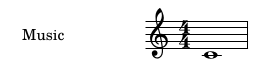
\includegraphics{HelloWorld.png}

\begin{lstlisting}[language=XML, caption ={HelloWorld.xml}]
<?xml version="1.0" encoding="UTF-8" standalone="no"?>
<!DOCTYPE score-partwise PUBLIC
    "-//Recordare//DTD MusicXML 3.0 Partwise//EN"
    "http://www.musicxml.org/dtds/partwise.dtd">
<score-partwise version="3.0">
  <!-- A very minimal MusicXML example -->
  <part-list>
    <score-part id="P1">
      <part-name>Music</part-name>
    </score-part>
  </part-list>
  <part id="P1">
<!--=========================================================-->
    <measure number="1">
  <!-- A very minimal MusicXML example, part P1, measure 1 -->
      <attributes>
        <divisions>1</divisions>
        <key>
          <fifths>0</fifths>
        </key>
        <time>
          <beats>4</beats>
          <beat-type>4</beat-type>
        </time>
        <clef>
          <sign>G</sign>
          <line>2</line>
        </clef>
      </attributes>
  <!-- A very minimal MusicXML example, part P1, measure 1, before first note -->
      <note>
        <pitch>
          <step>C</step>
          <octave>4</octave>
        </pitch>
        <duration>4</duration>
        <type>whole</type>
      </note>
    </measure>
<!--=========================================================-->
  </part>
</score-partwise>
\end{lstlisting}
%\end{figure}


% -------------------------------------------------------------------------
% -------------------------------------------------------------------------
\section{Score structure}
% -------------------------------------------------------------------------
% -------------------------------------------------------------------------

\mxml\ data contains a mix of legal informations, score geometry and musical contents. Some aspects of this are presented in this section.

% -------------------------------------------------------------------------
\subsection{Identification and rights}
% -------------------------------------------------------------------------

The '{\tt  <identification>}' element is defined in \schemafile{identity.mod}:
\begin{lstlisting}[language=XML]
<!--
	Identification contains basic metadata about the score.
	It includes the information in MuseData headers that
	may apply at a score-wide, movement-wide, or part-wide
	level. The creator, rights, source, and relation elements
	are based on Dublin Core.
-->
<!ELEMENT identification (creator*, rights*, encoding?,
	source?, relation*, miscellaneous?)>

<!--
	The creator element is borrowed from Dublin Core. It is
	used for the creators of the score. The type attribute is
	used to distinguish different creative contributions. Thus,
	there can be multiple creators within an identification.
	Standard type values are composer, lyricist, and arranger.
	Other type values may be used for different types of
	creative roles. The type attribute should usually be used
	even if there is just a single creator element. The MusicXML
	format does not use the creator / contributor distinction
	from Dublin Core.
-->
<!ELEMENT creator (#PCDATA)>
<!ATTLIST creator
    type CDATA #IMPLIED
>
\end{lstlisting}

For example, \mxmlfile{xmlsamples3.1/ActorPreludeSample.xml} contains:
\begin{lstlisting}[language=XML,caption={Identification and rights example}]
  <identification>
    <creator type="composer">Lee Actor</creator>
    <rights>© 2004 Polygames.     All Rights Reserved.</rights>
    <encoding>
      <software>Finale v25 for Mac</software>
      <encoding-date>2017-12-12</encoding-date>
      <supports attribute="new-system" element="print" type="yes" value="yes"/>
      <supports attribute="new-page" element="print" type="yes" value="yes"/>
      <supports element="accidental" type="yes"/>
      <supports element="beam" type="yes"/>
      <supports element="stem" type="yes"/>
    </encoding>
  </identification>
\end{lstlisting}

% -------------------------------------------------------------------------
\subsection{Score geometry}
% -------------------------------------------------------------------------

The dimensions and margins of the graphics score can be specified with the '{\tt <page-layout>}' element, as in \mxmlfile{basic/ClefKeyTime.xml}:
\begin{lstlisting}[language=XML, caption={Page layout example}]
  <defaults>
    <scaling>
      <millimeters>7.05556</millimeters>
      <tenths>40</tenths>
      </scaling>
    <page-layout>
      <page-height>1683.36</page-height>
      <page-width>1190.88</page-width>
      <page-margins type="even">
        <left-margin>56.6929</left-margin>
        <right-margin>56.6929</right-margin>
        <top-margin>56.6929</top-margin>
        <bottom-margin>113.386</bottom-margin>
        </page-margins>
      <page-margins type="odd">
        <left-margin>56.6929</left-margin>
        <right-margin>56.6929</right-margin>
        <top-margin>56.6929</top-margin>
        <bottom-margin>113.386</bottom-margin>
        </page-margins>
      </page-layout>
    <word-font font-family="FreeSerif" font-size="10"/>
    <lyric-font font-family="FreeSerif" font-size="11"/>
    </defaults>
\end{lstlisting}

% -------------------------------------------------------------------------
\subsection{Part groups and parts}
% -------------------------------------------------------------------------

Part groups are used to structure complex scores, mimicking the way large orchestras are organized. For example, there can be a winds group, containing several groups such as flutes, oboes, horns and bassoons.

A '{\tt <part-group>}' element has a '{\tt type}' attribute, whose value can be '{\tt start}' or '{\tt stop}'. A~part group is thus delimited by a pair of '{\tt <part-group>}' elements, the first one of type '{\tt start}', and the second one of type '{\tt stop}'.

The '{\tt id}' attribute of the '{\tt <score-part>}' element is used to reference the part later in the \mxml\ data. Often, is has the form '{\tt Pn}', where '{\tt n}' is a number.

Part groups can be nested, leading to a hierarchy of groups. This is done with the '{\tt number}' attribute of the '{\tt <part-group>}' element, which indicates how '{\tt start}' and '{\tt stop}' attributes are paired together.

For example, \mxmlfile{partgroups/NestedPartGroups.xml} contains:

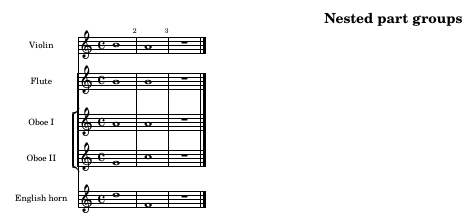
\includegraphics{NestedPartGroups.png}

\begin{lstlisting}[language=XML, caption={Nested part groups example}]
  <part-list>
    <score-part id="P1">
      <part-name>Violin</part-name>
    </score-part>
    <part-group number="1" type="start">
      <group-symbol>line</group-symbol>
      <group-barline>yes</group-barline>
    </part-group>
    <score-part id="P2">
      <part-name>Flute</part-name>
    </score-part>
    <part-group number="2" type="start">
      <group-symbol>bracket</group-symbol>
      <group-barline>yes</group-barline>
    </part-group>
    <score-part id="P3">
      <part-name>Oboe I</part-name>
    </score-part>
    <score-part id="P4">
      <part-name>Oboe II</part-name>
    </score-part>
    <part-group number="2" type="stop"/>
    <part-group number="1" type="stop"/>
    <score-part id="P5">
      <part-name>English horn</part-name>
    </score-part>
  </part-list>
\end{lstlisting}

The \mxml\ DTD states that part groups may {\it overlap}. This seem to be only because \fin\ doesn't create \mxml\ markups in a strict first-in, last-out order.

Here is how \mxmlfile{partgroups/OverlappingPartGroups.xml} is handled by various applications:

\begin{itemize}
\item \sib\ 7.1.3 loses the last group, i.e. the bassoons;
\item \fin\ 2014 loses them too;
\item \muse\ 3.3.4 crashes;
\item \mxmlToLy\ loses the bassoons too;
\item \xmlToLy\ rejects such data for the time being, with the message shown below.
\end{itemize}

\begin{lstlisting}[language=XML]
  ### MusicXML ERROR ### partgroups/OverlappingPartGroups.xml:169: 
There are overlapping part groups, namely: 
  '2' -=> PartGroup_6 ('2', partGroupName "1
2"), lines 164..169
and
  '1' -=> PartGroup_2 ('1', partGroupName ""), lines 76..170

Please contact the maintainers of libmusicxml2 (see option '-c, -contact'):
  either you found a bug in the xml2ly translator,
  or this MusicXML data is the first-ever real-world case
  of a score exhibiting overlapping part groups.
Abort trap: 6 (core dumped)
\end{lstlisting}


% -------------------------------------------------------------------------
\subsection{Staves and voices}
% -------------------------------------------------------------------------

In \mxml, a part is composed of one or more staves, each composed of one or more voices. 
There are no structured staves nor voices in \mxml\ however -- the way parts and measures are. The '{\tt <stave>}' and '{\tt voice}' element only contain a number.

To be more precise:
\begin{itemize}
\item stave numbers start at 1 in every part, which refers to the top-most staff in the part;

\item a stave number of 1 is implied by default, i.e. when an optional '{\tt <stave>}' element is missing, as can happen in notes descriptions;

\item voice numbers start at 1 in every staff, and a voice number of 1 is implied by default, i.e. when an optional '{\tt <voice>}' element is missing;
\end{itemize}

This author has found \mxml\ files in which the voice numbers are not contiguous, such as 1, 5, 9. The DTD doesn't preclude this. The way \mxmlfile{multistaff/NonContiguousVoiceNumbers.xml} is handled depends on the application.

A given voice can change staff and come back to the former one, for example in keyboard scores.

% -------------------------------------------------------------------------
\subsection{Clefs, keys and time signatures}
% -------------------------------------------------------------------------

\mxml\ offers elements to describe the common cases:
\begin{itemize}
\item traditional keys are described by a '{\tt <fifths>}' element;

\item simple clefs are described by '{\tt <sign>}' and '{\tt <line>}' elements;

\item simple time signatures are desribed by '{\tt <beats>}' and '{\tt <beat-type>}' elements.
\end{itemize}

An example is found in \mxmlfile{basic/ClefKeyTime.xml}:

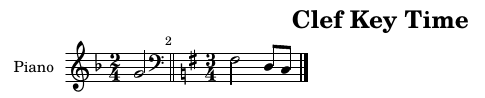
\includegraphics{ClefKeyTime.png}

\begin{lstlisting}[language=XML, caption={Clef, key and time signature example}]
      <attributes>
        <divisions>2</divisions>
        <key>
          <fifths>-1</fifths>
          </key>
        <time>
          <beats>2</beats>
          <beat-type>4</beat-type>
          </time>
        <clef>
          <sign>G</sign>
          <line>2</line>
          </clef>
        </attributes>
      <!-- ... ... ... ... ... -->
      <attributes>
        <key>
          <fifths>1</fifths>
          </key>
        <time>
          <beats>3</beats>
          <beat-type>4</beat-type>
          </time>
        <clef>
          <sign>F</sign>
          <line>4</line>
          </clef>
        </attributes>
\end{lstlisting}

In this example, the various sub-elements are:
%\begin{adjustwidth}{-0.5cm}{-0.5cm}
\begin{center}
\footnotesize
\def \contentsWidth{0.5\textwidth}
\def \arraystretch{1.3}
%
\begin{tabular}[t]{lp{\contentsWidth}}
\textbf{Fragment}&\textbf{Meaning} \tabularnewline[0.5ex]
\hline\\[-3.0ex]
%
'{\tt  <fifths>-1</fifths>}' & the number of fitfhs. A negative number is the number of flats, 0 means C major or A minor, and a positive value is the number of sharps
\tabularnewline

'{\tt <beats>2</beats>}' & the number of beats per measure \tabularnewline

'{\tt <beat-type>4</beat-type>}' & the beat type, i.e. the duration of each beat expressed as a fraction of a whole note
\tabularnewline

'{\tt <sign>G</sign>}' & the clef sign to be displayed. Sign values include '{\tt G}', '{\tt F}', '{\tt C}',
	'{\tt percussion}', '{\tt TAB}', '{\tt jianpu}', and '{\tt none}'
\tabularnewline

'{\tt <line>2</line>}' & the number of the line at which the clef is placed
\tabularnewline

\end{tabular}
\end{center}
%\end{adjustwidth}

Composite time signatures such as '{\tt 2/4 + 3/8}' and '{\tt 3+2/8}' can be specified, as well as '{\tt <senza-misura>}' for cadenzas.

\mxml\ also supports non-traditional keys the Humdrum/Scot way. For example, the time signature at the beginning of measure 2 in \mxmlfile{keys/HumdrumScotKeys.xml} is described by:

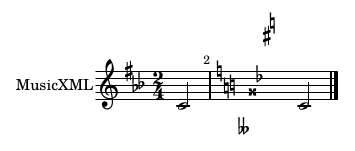
\includegraphics{HumdrumScotKeys.png}
 
\begin{lstlisting}[language=XML, caption={Humdrum/Scot non-traditional key example}]
        <key>
          <key-step>C</key-step>
          <key-alter>-2</key-alter>
          <key-step>G</key-step>
          <key-alter>2</key-alter>
          <key-step>D</key-step>
          <key-alter>-1</key-alter>
          <key-step>B</key-step>
          <key-alter>1</key-alter>
          <key-step>F</key-step>
          <key-alter>0</key-alter>
          <key-octave number="1">2</key-octave>
          <key-octave number="2">3</key-octave>
          <key-octave number="3">4</key-octave>
          <key-octave number="4">5</key-octave>
          <key-octave number="5">6</key-octave>
        </key>
\end{lstlisting}

This is another example handled diffently by some applications.

% -------------------------------------------------------------------------
\subsection{Metromone and tempo}
% -------------------------------------------------------------------------

% -------------------------------------------------------------------------
\subsection{Measures}
% -------------------------------------------------------------------------

The '{\tt <measure>}' elements can contain many other elements, depending on the music.

Full measures are usually numbered from '{\tt 1}' up, but these numbers are actually character strings, not integers: this allows for special measure numbers such as '{\tt X1}', for example, in the case of cue staves.

Anacruses are best specified with '{\tt 0}' as their number and the '{\tt implicit}' attribute set to '{\tt yes}':
\begin{lstlisting}[language=XML]
    <measure number="0" implicit="yes" width="129.48">
\end{lstlisting}

One see cases where the number is 1 for anacruses, though.

Measure can be much longer that the usual time signagures, see \ref{lyrics}.

Staves have numbers from '{\tt 1}' up, with stave number '{\tt 1}' the top-most one in a given part.

% -------------------------------------------------------------------------
\subsection{'{\tt <forward>}' and '{\tt <backup>}}'\label{forwardAndBackup}%\ContentsLabel{NAT}
% -------------------------------------------------------------------------

The '{\tt <forward>}' element is used typically in a second, third or fourth voice which does not contain notes at some point in time. This element allows drawing to continue a bit further in the voice, without drawing rests in-between.

The '{\tt <backup>}' is needed to move to the left before drawing the next element. This is necessary where there are several voices in a given staff and one switched drawing from one voice to another, whose next element is not at the right of the last one drawn.


% -------------------------------------------------------------------------
% -------------------------------------------------------------------------
\section{Notes}
% -------------------------------------------------------------------------
% -------------------------------------------------------------------------

A note is described by a '{\tt note}' element, defined in \schemafile{note.mod}:
\begin{lstlisting}[language=XML, caption={Note definition}]
<!--
	Notes are the most common type of MusicXML data. The
	MusicXML format keeps the MuseData distinction between
	elements used for sound information and elements used for
	notation information (e.g., tie is used for sound, tied for
	notation). Thus grace notes do not have a duration element.
	Cue notes have a duration element, as do forward elements,
	but no tie elements. Having these two types of information
	available can make interchange considerably easier, as
	some programs handle one type of information much more
	readily than the other.
-->
<!ELEMENT note
	(((grace, ((%full-note;, (tie, tie?)?) | (cue, %full-note;))) |
	  (cue, %full-note;, duration) |
	  (%full-note;, duration, (tie, tie?)?)),
	 instrument?, %editorial-voice;, type?, dot*,
	 accidental?, time-modification?, stem?, notehead?,
	 notehead-text?, staff?, beam*, notations*, lyric*, play?)>
\end{lstlisting}


The first note in measure 2 in \mxmlfile{basic/MinimalScore.xml}:

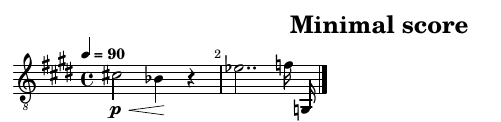
\includegraphics{MinimalScore.png}

is described by:
\begin{lstlisting}[language=XML, caption ={Note example}]
        <divisions>8</divisions>
        
      <!-- ... ... ... ... ... -->
      
        <clef>
          <sign>G</sign>
          <line>2</line>
          <clef-octave-change>-1</clef-octave-change>
        </clef>

      <!-- ... ... ... ... ... -->
      
      <note>
        <pitch>
          <step>E</step>
          <alter>-1</alter>
          <octave>4</octave>
        </pitch>
        <duration>28</duration>
        <voice>1</voice>
        <type>half</type>
        <dot />
        <dot />
        <accidental>flat</accidental>
      </note>
\end{lstlisting}

In this example, the various sub-elements are:
%\begin{adjustwidth}{-0.5cm}{-0.5cm}
\begin{center}
\footnotesize
\def \contentsWidth{0.5\textwidth}
\def \arraystretch{1.3}
%
\begin{tabular}[t]{lp{\contentsWidth}}
\textbf{Fragment}&\textbf{Meaning} \tabularnewline[0.5ex]
\hline\\[-3.0ex]
%
'{\tt <step>E</step>}' & the diatonic pitch of the note, from A to G
\tabularnewline

'{\tt <alter>-1</alter>}' & the chromatic alteration in
	number of semitones (e.g., -1 for flat, 1 for sharp)
\tabularnewline

'{\tt <octave>4</octave>}' & the absolute octave of the note, 0 to 9, where 4 indicates the octave
	started by middle C
\tabularnewline

'{\tt <duration>28</duration>}' & the sounding duration of the note, 28 quanta, which is a double dotted half note with 4 quanta per quarter note (16+8+4)
\tabularnewline

'{\tt <voice>1</voice>}' & the voice number of the note, 1
\tabularnewline

'{\tt <type>half</type>}' & the display duration of the note, a half note, which determines the note head
\tabularnewline

\end{tabular}
\end{center}
%\end{adjustwidth}

Middle C is the one between the left hand and right hand staves in a typical score. Note here: octave numbers are absolute, and the treble clef is octaviated by a '{\tt <clef-octave-change>}' element!

Voice and staff numbers are optional, in which case the default value is 1.

Having both a sounding and display duration specification is necessary because they do not coincide in the case of dotted notes and tuplets members, see paragraph \ref{tuplets} for the latter.

% -------------------------------------------------------------------------
\subsection{Accidentals}
% -------------------------------------------------------------------------

\begin{lstlisting}[language=XML]
<!--
	Actual notated accidentals. Valid values include: sharp,
	natural, flat, double-sharp, sharp-sharp, flat-flat,
	natural-sharp, natural-flat, quarter-flat, quarter-sharp,
	three-quarters-flat, three-quarters-sharp, sharp-down,
	sharp-up, natural-down, natural-up, flat-down, flat-up,
	double-sharp-down, double-sharp-up, flat-flat-down,
	flat-flat-up, arrow-down, arrow-up, triple-sharp,
	triple-flat, slash-quarter-sharp, slash-sharp, slash-flat,
	double-slash-flat, sharp-1, sharp-2, sharp-3, sharp-5,
	flat-1, flat-2, flat-3, flat-4, sori, koron, and other.

	The quarter- and three-quarters- accidentals are
	Tartini-style quarter-tone accidentals. The -down and -up
	accidentals are quarter-tone accidentals that include
	arrows pointing down or up. The slash- accidentals
	are used in Turkish classical music. The numbered
	sharp and flat accidentals are superscripted versions
	of the accidental signs, used in Turkish folk music.
	The sori and koron accidentals are microtonal sharp and
	flat accidentals used in Iranian and Persian music. The
	other accidental covers accidentals other than those listed
	here. It is usually used in combination with the smufl
	attribute to specify a particular SMuFL accidental. The
	smufl attribute may be used with any accidental value to
	help specify the appearance of symbols that share the same
	MusicXML semantics. The attribute value is a SMuFL canonical
	glyph name that starts with acc.

	Editorial and cautionary indications are indicated
	by attributes. Values for these attributes are "no" if not
	present. Specific graphic display such as parentheses,
	brackets, and size are controlled by the level-display
	entity defined in the common.mod file.
-->
<!ELEMENT accidental (#PCDATA)>
<!ATTLIST accidental
    cautionary %yes-no; #IMPLIED
    editorial %yes-no; #IMPLIED
    %level-display;
    %print-style;
    %smufl;
>
\end{lstlisting}

% -------------------------------------------------------------------------
\subsection{Articulations}
% -------------------------------------------------------------------------
The \mxml\ articulation elementss are:
\begin{lstlisting}[language=XML]
<!--
	Articulations and accents are grouped together here.
-->
<!ELEMENT articulations
	((accent | strong-accent | staccato | tenuto |
	  detached-legato | staccatissimo | spiccato |
	  scoop | plop | doit | falloff | breath-mark |
	  caesura | stress | unstress | soft-accent |
	  other-articulation)*)>
<!ATTLIST articulations
    %optional-unique-id;
>
\end{lstlisting}

% -------------------------------------------------------------------------
\subsection{Ornaments}
% -------------------------------------------------------------------------

Ornaments are defined in \schemafile{note.mod}:
\begin{lstlisting}[language=XML]
<!--
	Ornaments can be any of several types, followed optionally
	by accidentals. The accidental-mark element's content is
	represented the same as an accidental element, but with a
	different name to reflect the different musical meaning.
-->
<!ELEMENT ornaments
	(((trill-mark | turn | delayed-turn | inverted-turn |
	   delayed-inverted-turn | vertical-turn |
	   inverted-vertical-turn | shake | wavy-line |
	   mordent | inverted-mordent | schleifer | tremolo |
	   haydn | other-ornament), accidental-mark*)*)>
<!ATTLIST ornaments
    %optional-unique-id;
>
<!ELEMENT trill-mark EMPTY>
<!ATTLIST trill-mark
    %print-style;
    %placement;
    %trill-sound;
>
\end{lstlisting}

% -------------------------------------------------------------------------
\subsection{Dynamics}
% -------------------------------------------------------------------------

\mxml\ dynamics are defined in \schemafile{common.mod}:

\begin{lstlisting}[language=XML]
<!ELEMENT dynamics ((p | pp | ppp | pppp | ppppp | pppppp |
	f | ff | fff | ffff | fffff | ffffff | mp | mf | sf |
	sfp | sfpp | fp | rf | rfz | sfz | sffz | fz | 
	n | pf | sfzp | other-dynamics)*)>
<!ATTLIST dynamics
    %print-style-align; 
    %placement;
    %text-decoration; 
    %enclosure;
    %optional-unique-id;
\end{lstlisting}

Other dynamics can also be specified:
\begin{lstlisting}[language=XML]
The other-dynamics element
	allows other dynamic marks that are not covered here, but
	many of those should perhaps be included in a more general
	musical direction element. Dynamics may also be combined as
	in <sf/><mp/>.
\end{lstlisting}

% -------------------------------------------------------------------------
\subsection{Grace notes}
% -------------------------------------------------------------------------

The '{\tt <grace>}' element is defined in \schemafile{note.mod}:
\begin{lstlisting}[language=XML]
<!--
	The grace element indicates the presence of a grace note. 
	The slash attribute for a grace note is yes for slashed
	eighth notes. The other grace note attributes come from
	MuseData sound suggestions. The steal-time-previous attribute
	indicates the percentage of time to steal from the previous
	note for the grace note. The steal-time-following attribute
	indicates the percentage of time to steal from the following
	note for the grace note, as for appoggiaturas. The make-time
	attribute indicates to make time, not steal time; the units
	are in real-time divisions for the grace note.
-->
<!ELEMENT grace EMPTY>
<!ATTLIST grace
    steal-time-previous CDATA #IMPLIED
    steal-time-following CDATA #IMPLIED
    make-time CDATA #IMPLIED
    slash %yes-no; #IMPLIED
>
\end{lstlisting}

% -------------------------------------------------------------------------
% -------------------------------------------------------------------------
\section{Ties and slurs}
% -------------------------------------------------------------------------
% -------------------------------------------------------------------------

From \schemafile{note.mod}:

\begin{lstlisting}[language=XML]
<!--
	The tied element represents the notated tie. The tie element
	represents the tie sound.

	The number attribute is rarely needed to disambiguate ties,
	since note pitches will usually suffice. The attribute is
	implied rather than defaulting to 1 as with most elements. It is
	available for use in more complex tied notation situations.

	Ties that join two notes of the same pitch together should be
	represented with a tied element on the first note with
	type="start" and a tied element on the second note with
	type="stop".  This can also be done if the two notes being tied
	are enharmonically equivalent, but have different step values. It
	is not recommended to use tied elements to join two notes with
	enharmonically inequivalent pitches.

	Ties that indicate that an instrument should be undamped are
	specified with a single tied element with type="let-ring".

	Ties that are visually attached to only one note, other than
	undamped ties, should be specified with two tied elements on the
	same note, first type="start" then type="stop". This can be used
	to represent ties into or out of repeated sections or codas.
-->
<!ELEMENT tied EMPTY>
<!ATTLIST tied
    type %tied-type; #REQUIRED
    number %number-level; #IMPLIED
    %line-type;
    %dashed-formatting;
    %position;
    %placement;
    %orientation;
    %bezier;
    %color;
    %optional-unique-id;
>
\end{lstlisting}

The '{\tt <tie>}' element

The '{\tt <tied>}' element


The '{\tt <slur>}' element is placed inside a '{\tt <notations>}' element, itself placed inside a '{\tt <note>}' element. Is has two attributes:
\begin{enumerate}
\item '{\tt type}' can contain '{\tt start}' or '{\tt stop}';
\item '{\tt number}' allows for nested slurs.
\end{enumerate}

An example can be seen in \mxmlfile{basic/TieAndSlur.xml}:

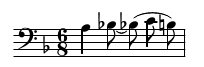
\includegraphics{TieAndSlur.png}
\begin{lstlisting}[language=XML, caption={Tie and slur example}]
      <note>
        <pitch>
          <step>A</step>
          <octave>3</octave>
        </pitch>
        <duration>2</duration>
        <type>quarter</type>
        <voice>1</voice>
      </note>
      <note>
        <pitch>
          <step>B</step>
          <alter>-1</alter>
          <octave>3</octave>
        </pitch>
        <duration>1</duration>
        <type>eighth</type>
        <voice>1</voice>
        <accidental>flat</accidental>
        <tie type="start" />
        <notations>
          <tied type="start" />
        </notations>
      </note>
      <note>
        <pitch>
          <step>B</step>
          <alter>-1</alter>
          <octave>3</octave>
        </pitch>
        <duration>1</duration>
        <type>eighth</type>
        <voice>1</voice>
        <accidental>flat</accidental>
        <tie type="stop" />
        <notations>
          <tied type="stop" />
          <slur number="1" type="start" />
        </notations>
      </note>
      <note>
        <pitch>
          <step>C</step>
          <octave>4</octave>
        </pitch>
        <duration>1</duration>
        <type>eighth</type>
        <voice>1</voice>
      </note>
      <note>
        <pitch>
          <step>B</step>
          <octave>3</octave>
        </pitch>
        <duration>1</duration>
        <type>eighth</type>
        <voice>1</voice>
        <notations>
          <slur number="1" type="stop" />
        </notations>
      </note>
\end{lstlisting}

% -------------------------------------------------------------------------
% -------------------------------------------------------------------------
\section{Harmonies and figured bass}
% -------------------------------------------------------------------------
% -------------------------------------------------------------------------

% -------------------------------------------------------------------------
% -------------------------------------------------------------------------
\section{Chords and tuplets}
% -------------------------------------------------------------------------
% -------------------------------------------------------------------------

% -------------------------------------------------------------------------
\subsection{Chords}
% -------------------------------------------------------------------------

Chords are not evidenced as such in \mxml\ data. Instead, the '{\tt <chord>}' element means that the given note is part of a chord after the first note in the chord has be met. Remember:~\mxml\ is about drawing scores. Put it another way, you know there is a chord upon its second note.

The code for the last three note chord in \mxmlfile{chords/Chords.xml} is shown below.

%\begin{figure}
%\caption{Last chord from \mxmlfile{chords/Chords.xml}\label{chords}
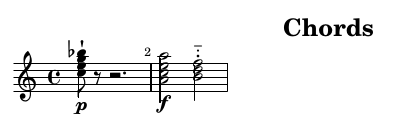
\includegraphics{Chords.png}

\begin{lstlisting}[language=XML, caption={Chord example}]
      <note>
        <pitch>
          <step>B</step>
          <octave>4</octave>
        </pitch>
        <duration>4</duration>
        <voice>1</voice>
        <type>half</type>
        <notations>
          <articulations>
            <staccato />
            <detached-legato />
          </articulations>
        </notations>
      </note>
      <note>
        <chord />
        <pitch>
          <step>D</step>
          <octave>5</octave>
        </pitch>
        <duration>4</duration>
        <voice>1</voice>
        <type>half</type>
      </note>
      <note>
        <chord />
        <pitch>
          <step>F</step>
          <octave>5</octave>
        </pitch>
        <duration>4</duration>
        <voice>1</voice>
        <type>half</type>
      </note>
\end{lstlisting}
%\end{figure}

% -------------------------------------------------------------------------
\subsection{Tuplets}\label{tuplets}
% -------------------------------------------------------------------------

The situation for tuplets is different than that of the chords: there is a '{\tt <tuplet>}' element, with a '{\tt type}' attribute to indicate the note upon which it starts and stops:

\begin{lstlisting}[language=XML]
        <notations>
          <tuplet number="1" type="start" />
        </notations>
\end{lstlisting}

The '{\tt number}' attribute can be used to describe nested tuplets:

The contents, i.e. the notes in the tuplet, are not nested in the latter: there are placed in sequence between the two '{\tt <tuplet>}' elements that delimitate the tuplet. 

Each note in the tuplet has a '{\tt <time-modification>}' element, from the first one on. This element contains two elements:
\begin{lstlisting}[language=XML]
        <time-modification>
          <actual-notes>3</actual-notes>
          <normal-notes>2</normal-notes>
        </time-modification>
\end{lstlisting}

One should play '{\tt <actual-notes>}' within the time taken by only '{\tt <normal-notes>}'. The example above is thus that of a triplet.

In the case of \mxmlfile{tuplets/Tuplets.xml}, shown below, the duration of the tuplets member is 20 quanta, i.e. 2/3 of a quarter note, whose duration is 30, and the 'display' duration is a quarter note. The duration of the triplet as a whole is that of a half note, i.e. 60 quanta.

%\begin{figure}
%\caption{First tuplet from \mxmlfile{tuplets/Tuplet.xml}}\label{tuplets}
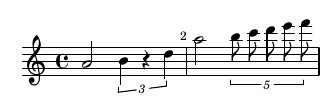
\includegraphics{Tuplet.png}

\begin{lstlisting}[language=XML, caption={Tuplet example}]
        <divisions>30</divisions>

			<!-- ... ... ... ... ... -->
			
      <note>
        <pitch>
          <step>B</step>
          <octave>4</octave>
        </pitch>
        <duration>20</duration>
        <voice>1</voice>
        <type>quarter</type>
        <time-modification>
          <actual-notes>3</actual-notes>
          <normal-notes>2</normal-notes>
        </time-modification>
        <notations>
          <tuplet number="1" type="start" />
        </notations>
      </note>
      <note>
        <rest />
        <duration>20</duration>
        <voice>1</voice>
        <type>quarter</type>
        <time-modification>
          <actual-notes>3</actual-notes>
          <normal-notes>2</normal-notes>
        </time-modification>
      </note>
      <note>
        <pitch>
          <step>D</step>
          <octave>5</octave>
        </pitch>
        <duration>20</duration>
        <voice>1</voice>
        <type>quarter</type>
        <time-modification>
          <actual-notes>3</actual-notes>
          <normal-notes>2</normal-notes>
        </time-modification>
        <notations>
          <tuplet number="1" type="stop" />
        </notations>
      </note>
\end{lstlisting}
%\end{figure}


% -------------------------------------------------------------------------
% -------------------------------------------------------------------------
\section{Barlines and repeats}
% -------------------------------------------------------------------------
% -------------------------------------------------------------------------

Repeats are not described by high-level elements in \mxml. Instead, specific barlines containing a '{\tt <repeat>}' element are used to draw the necessary delimiters.

% -------------------------------------------------------------------------
\subsection{Simple barlines}
% -------------------------------------------------------------------------

The '{\tt <barline>}' element is defined in \schemafile{barline.mod}. It has two main attributes:
%\begin{adjustwidth}{-0.5cm}{-0.5cm}
\begin{center}
\footnotesize
\def \contentsWidth{0.5\textwidth}
\def \arraystretch{1.3}
%
\begin{tabular}[t]{lp{\contentsWidth}}
\textbf{Attribute}&\textbf{Meaning} \tabularnewline[0.5ex]
\hline\\[-3.0ex]
%
{\tt bar-style} & Bar-style contains style information. Choices are
	'{\tt regular}', '{\tt dotted}', '{\tt dashed}', '{\tt heavy}', '{\tt light-light}', 
	'{\tt light-heavy}', '{\tt heavy-light}', '{\tt heavy-heavy}', '{\tt tick}' (a
	short stroke through the top line), '{\tt short}' (a partial
	barline between the 2nd and 4th lines), and '{\tt none}'.

	Barlines can occur within measures, as in dotted
	barlines that subdivide measures in complex meters;
\tabularnewline

{\tt location} & If location is '{\tt left}',
	it should be the first element in the measure, aside from
	the '{\tt print}', '{\tt bookmark}', and '{\tt link}' elements. 
	
	If location is
	'{\tt right}', it should be the last element, again with the
	possible exception of the '{\tt print}', '{\tt bookmark}', and '{\tt link}'
	elements.
	
	The value can be '{\tt right}', '{\tt left}' or '{\tt middle}'.
	If no location is specified, the default value is '{\tt right}'.
\tabularnewline

\end{tabular}
\end{center}
%\end{adjustwidth}

%The possible bar styles are defined in \schemafile{barline.mod}:
%\begin{lstlisting}[language=XML,caption={Existing bar styles}]
%<!--
%	Bar-style contains style information. Choices are
%	regular, dotted, dashed, heavy, light-light, 
%	light-heavy, heavy-light, heavy-heavy, tick (a
%	short stroke through the top line), short (a partial
%	barline between the 2nd and 4th lines), and none.
%-->
%<!ELEMENT bar-style (#PCDATA)>
%<!ATTLIST bar-style
%  %color;
%>
%\end{lstlisting}
%

In the '{\tt <bar-style>}' element, '{\tt light}' is a thin vertical line, and '{\tt heavy}'is a thick line. The final barline of a piece is thus represented by:
\begin{lstlisting}[language=XML, caption={Final barline}]
      <barline location="right">
        <bar-style>light-heavy</bar-style>
        </barline>
\end{lstlisting}

One can see the various simple barlines in \mxmlfile{barlines/SimpleBarlines.xml}:

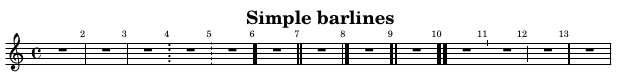
\includegraphics{SimpleBarlines.png}

% -------------------------------------------------------------------------
\subsection{Repeats}
% -------------------------------------------------------------------------

The '{\tt <repeat>}' element in barline can contains these attributes, also defined in \schemafile{barline.mod}:
%\begin{adjustwidth}{-0.5cm}{-0.5cm}
\begin{center}
\footnotesize
\def \contentsWidth{0.5\textwidth}
\def \arraystretch{1.3}
%
\begin{tabular}[t]{lp{\contentsWidth}}
\textbf{Attribute}&\textbf{Meaning} \tabularnewline[0.5ex]
\hline\\[-3.0ex]
%
{\tt direction} & '{\tt forward}' is used at the start of a repeat, and '{\tt backward}' is used at the end of it;
\tabularnewline

{\tt times} & indicates how many times the repeated section as to be played;
\tabularnewline

{\tt winged} & indicates whether	has winged extensions that appear above and below the barline, to make them easier to see;

The '{\tt straight}' and '{\tt curved}' values represent single wings, while
	the '{\tt double-straight}' and '{\tt double-curved}' values represent double
	wings. The '{\tt none}' value indicates no wings and is the default.
\tabularnewline

\end{tabular}
\end{center}
%\end{adjustwidth}

%\begin{lstlisting}[language=XML,caption={Repeats barlines}]
%<!--
%	Repeat marks. The start of the repeat has a forward direction
%	while the end of the repeat has a backward direction. Backward
%	repeats that are not part of an ending can use the times
%	attribute to indicate the number of times the repeated section
%	is played. The winged attribute indicates whether the repeat
%	has winged extensions that appear above and below the barline.
%	The straight and curved values represent single wings, while
%	the double-straight and double-curved values represent double
%	wings. The none value indicates no wings and is the default.
%-->
%<!ELEMENT repeat EMPTY>
%<!ATTLIST repeat
%    direction (backward | forward) #REQUIRED
%    times CDATA #IMPLIED
%    winged (none | straight | curved | 
%		double-straight | double-curved) #IMPLIED
%>
%\end{lstlisting}
%


\begin{lstlisting}[language=XML]
      <barline location="right">
        <bar-style>light-heavy</bar-style>
        <repeat direction="backward" times="5"/>
      </barline>
\end{lstlisting}

\begin{lstlisting}[language=XML]
    <barline location="right">
      <bar-style>light-heavy</bar-style>
      <repeat direction="backward" winged="none"/>
    </barline>
\end{lstlisting}


% -------------------------------------------------------------------------
% -------------------------------------------------------------------------
\section{Lyrics}\label{lyrics}
% -------------------------------------------------------------------------
% -------------------------------------------------------------------------

In \mxml\, the '{\tt <lyrics>}' elements are attached to the '{\tt <note>}' elements. The definition is in \schemafile{note.mod}:
\begin{lstlisting}[language=XML]
<!ELEMENT lyric
	((((syllabic?, text),
	   (elision?, syllabic?, text)*, extend?) |
	   extend | laughing | humming),
	  end-line?, end-paragraph?, %editorial;)>
<!ATTLIST lyric
    number NMTOKEN #IMPLIED
    name CDATA #IMPLIED
    %justify;
    %position;
    %placement;
    %color;
    %print-object;
    %time-only;
    %optional-unique-id;
>
\end{lstlisting}

For example, \mxmlfile{QuemQueritis.xml} contains:

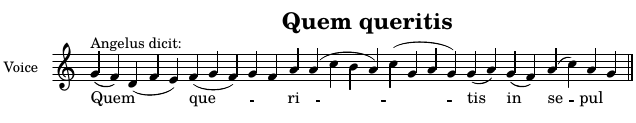
\includegraphics{QuemQueritis.png}
\begin{lstlisting}[language=XML]

\end{lstlisting}

% -------------------------------------------------------------------------
% -------------------------------------------------------------------------
\section{Creating \mxml\ data}
% -------------------------------------------------------------------------
% -------------------------------------------------------------------------

This can be done in various ways:
\begin{itemize}
\item by hand, using a text editor: possible, but unrealistic for usual scores;
\item by exporting the score as an \mxml\ text file with a GUI music score editor;
\item by scanning a graphics files containing a ready-to-print score, with tools such as PhotoScore Ultimate\texttrademark;
\item by programming an application that outputs \mxml\ text.
\end{itemize}

This author has performed manual text editing on some of the samples supplied with \lib\ in order to perform tests and debug \xmlToLy, but this is a particular case.

Exporting to \mxml\ is probably the most frequent way, and there are applications that do a good job at that. If an application supports say strings instruments scordaturas in scores, then creating a '{\tt <scordatura>}' element is not very difficult.

Scanning graphical scores is a tough problem:  how do you tell lyrics from annotations such as '{\tt cresc.}' or tempos such as '{\tt Allegro}'? One usually has to manually fix scanning errors and the category of some text fragments after scanning to get good results. And, then, the scanning application should create quality \mxml\ data.

Creating \mxml\ by an application is a matter of computer programming, and requires development skill. As an example, \lib\ supplies the necessary tools, and one can obtain:

\begin{lstlisting}[language=XML]
       <attributes>
        <key>
          <fifths>-1</fifths>
          </key>
        </attributes>
\end{lstlisting}

with C++ code such as:

\begin{lstlisting}[language=C++, caption ={Creating a key element in an application}]
  Sxmlelement attributes = factory::instance().create(k_attributes);

  Sxmlelement key = factory::instance().create(k_key);
  key->push (newElement(k_fifths, "1"));
  attributes->push (key);
\end{lstlisting}
 
% -------------------------------------------------------------------------
% -------------------------------------------------------------------------
\section{Importing \mxml\ data}
% -------------------------------------------------------------------------
% -------------------------------------------------------------------------

Many GUI applications provide a way to import \mxml\ data, often with some limitations. We show some of them here.

% -------------------------------------------------------------------------
\subsection{Small element, big effect}
% -------------------------------------------------------------------------

In \mxmlfile{harmonies/Inversion.xml}, shown below, there is a harmony with an '{\tt <inversion>}' element. A number of applications ignore this element when importing \mxml\ data, because it takes a full knowledge of chords structures to compute the bass note of inverted chords.
%\begin{figure}
%\caption{Harmony inversion from \mxmlfile{harmonies/Inversion.xml}}\label{inversion}
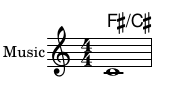
\includegraphics{Inversion.png}

\begin{lstlisting}[language=XML, caption = {Harmony inversion}]
      <harmony>
        <root>
          <root-step>F</root-step>
          <root-alter>1</root-alter>
        </root>
        <kind>major</kind>
        <inversion>2</inversion>
      </harmony>
\end{lstlisting}
%\end{figure}

% -------------------------------------------------------------------------
\subsection{Elements handled in different ways}
% -------------------------------------------------------------------------

% -------------------------------------------------------------------------
\subsection{Elements often not well handled}
% -------------------------------------------------------------------------

There are elements that are not displayed in a "standard" way by the usual music score editors. One of them is the '{\tt <beat-repeat>}'.


% -------------------------------------------------------------------------
\subsection{Elements usually not handled}
% -------------------------------------------------------------------------

There are elements that are not displayed by the usual music score editors, because there is no "standard" way to do so. One of them is the scordatura used on string instrument.

For example, the scordatura in \mxmlfile{strings/Scordatura.xml} is the case where the sixth string of the guitar is tuned a tone down to D, which can be described by:

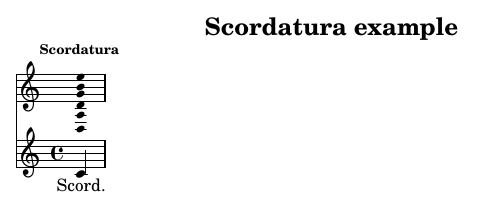
\includegraphics{Scordatura.png}

\begin{lstlisting}[language=XML, caption ={Scordatura example}]
          <scordatura>
              <accord string="6">
                <tuning-step>D</tuning-step>
                <tuning-alter>0</tuning-alter>
                <tuning-octave>3</tuning-octave>
              </accord>
              <accord string="5">
                <tuning-step>A</tuning-step>
                <tuning-alter>0</tuning-alter>
                <tuning-octave>3</tuning-octave>
              </accord>
              <accord string="4">
                <tuning-step>D</tuning-step>
                <tuning-alter>0</tuning-alter>
                <tuning-octave>4</tuning-octave>
              </accord>
              <accord string="3">
                <tuning-step>G</tuning-step>
                <tuning-alter>0</tuning-alter>
                <tuning-octave>4</tuning-octave>
              </accord>
              <accord string="2">
                <tuning-step>B</tuning-step>
                <tuning-alter>0</tuning-alter>
                <tuning-octave>4</tuning-octave>
              </accord>
              <accord string="1">
                <tuning-step>E</tuning-step>
                <tuning-alter>0</tuning-alter>
                <tuning-octave>5</tuning-octave>
              </accord>
          </scordatura>

\end{lstlisting}


% -------------------------------------------------------------------------
\subsection{A real challenge}
% -------------------------------------------------------------------------

The contents of \mxmlfile{challenging/BeethovenNinthSymphony.xml} is over 66 megabytes large. It was created by exporting it from \sib, and contains the whose score for this symphony. One can imagine the amount of work to create the score in the first place, and, of course, there's no way a human could create such \mxml\ data by hand.

The interested reader is urged to try and import this file in their favorite score editing sofware. This author's experience is that:

\begin{itemize}
\item \sib\ 7.1.3 handles it alright;
\item \fin\ 2014 finds it well-formed, but too big to be opened;
\item \muse\ 3.3 opens it, but then working on the file is extremely slow;
\item \mxmlToLy\ converts it to \lily\ syntax as of 2.19.83, and the result has some issues that should be fixed rather easily;
\item \xmlToLy\ converts it to \lily\ alright, but the issues in this case show that this converter is still experimental\dots
\end{itemize}

% -------------------------------------------------------------------------
% -------------------------------------------------------------------------
\section{Conclusion}
% -------------------------------------------------------------------------
% -------------------------------------------------------------------------

There is a lot of information about \mxml\ on the Internet. And of course, plenty of targeted, ready-to-use examples can be found in \subdir{files/samples/musicxml}.

\mxml\ has become a de facto standard for music scores data interchange between applications. As as been shown in this document, the way it is exported and imported by the various applications is quite diverse, and manual editing of the result is to be expected after import.
 
\mxml\ is not the whole story, though. The W3C Music Notation Community Group is working on MNX (\url{https://w3c.github.io/mnx}), as a successor to \mxml. One part of it is MNX-Common, which aims at being less verbose and more semantics-oriented than \mxml.

For example, consider:
\begin{lstlisting}[language=XML]
<score-partwise version="3.1">
    <part-list>
        <score-part id="P1">
            <part-name>Music</part-name>
        </score-part>
    </part-list>
    <part id="P1">
        <measure number="1">
            <attributes>
                <divisions>1</divisions>
                <key>
                    <fifths>0</fifths>
                </key>
                <time>
                    <beats>4</beats>
                    <beat-type>4</beat-type>
                </time>
                <clef>
                    <sign>G</sign>
                    <line>2</line>
                </clef>
            </attributes>
            <note>
                <pitch>
                    <step>C</step>
                    <octave>4</octave>
                </pitch>
                <duration>4</duration>
                <type>whole</type>
            </note>
        </measure>
    </part>
</score-partwise>
\end{lstlisting}

In MNX-Common, this can be written:
\begin{lstlisting}[language=XML,caption={MNX-Common example}]
<mnx>
    <score>
        <mnx-common profile="standard">
            <global>
                <measure>
                    <directions>
                        <time signature="4/4"/>
                    </directions>
                </measure>
            </global>
            <part>
                <part-name>Music</part-name>
                <measure barline="regular">
                    <sequence>
                        <directions>
                            <clef sign="G" line="2"/>
                        </directions>
                        <event value="/1">
                            <note pitch="C4"/>
                        </event>
                    </sequence>
                </measure>
            </part>
        </mnx-common>
    </score>
</mnx>
\end{lstlisting}

Let's conclude with a tribute to the manual score engravers, whose skills have produced so many beautiful scores for centuries! Reaching the quality of their work is still a challenge for current music scoring software.


% -------------------------------------------------------------------------
% -------------------------------------------------------------------------
% postamble
% -------------------------------------------------------------------------
% -------------------------------------------------------------------------

\pagebreak

\lstlistoflistings

%\listoffigures

\tableofcontents

% -------------------------------------------------------------------------
\end{document}
% -------------------------------------------------------------------------
